\documentclass[10pt,twocolumn,a4paper]{article}
\usepackage[margin=1in]{geometry} % Adjust margins for CVPR-like layout
\usepackage{times}
\usepackage{graphicx}
\usepackage{amsmath}
\usepackage{amssymb}
\usepackage{hyperref}
\usepackage{url}

\begin{document}

%%%%%%%%% TITLE
\title{Comparative Study on Stock Price Prediction Using RNN, LSTM, \& GRU}

\author{
    Shivangi \\
     The University of Adelaide\\
Adelaide, South Australia, Australia\\
{\tt\small shivangi@student.adelaide.edu.au}
}

\date{}
\maketitle

%%%%%%%%% ABSTRACT
\begin{abstract}
    Stock price prediction has always been a tough task as the financial market is too complex for accurate prediction. This research work compares Recurrent Neural Networks (RNN) and two of their variants, Long Short-Term Memory (LSTM) and Gated Recurrent Units (GRU), for short-term stock price trend prediction. The models were evaluated based on their Mean Squared Error (MSE) and validation loss. The study found that the LSTM model provided the best predictions. Furthermore, the LSTM model was used to forecast stock prices for an additional 30 days, demonstrating its superior performance in time-series forecasting.
\end{abstract}

%%%%%%%%% INTRODUCTION
\section{Introduction}
Financial planning and investment decisions make the most of stock price forecasting. However, traditional models such as ARIMA restrict their ability to model non-linear and complex dependencies inherent in financial time-series data. Recurrent Neural Networks (RNNs), particularly LSTM and GRU, are becoming popular as time-series forecasting techniques due to their capability in long-term dependency management. These models deal with sequence patterns in price movements for accurate predictions.

This study targets the following objectives:
\begin{itemize}
    \item To implement and compare RNN, LSTM, and GRU models for stock price prediction.
    \item To evaluate the performance of models using validation loss and Mean Squared Error (MSE).
    \item To upscale successful model prediction for future stock prices.
\end{itemize}

%%%%%%%%% BACKGROUND
\section{Background}
For predicting the stock prices, there are several approaches, from traditional statistical models to modern machine learning techniques. One such traditional model is ARIMA, which is commonly used for time-series forecasting. It assumes that the data follows a linear and stationary pattern, making it useful when the data follows simple trends. However, it struggles with stock prices because they often do not follow simple, linear patterns and are affected by long-term dependencies.

Similarly, GARCH models focus on predicting volatility rather than the actual stock prices. These models are better for understanding market fluctuations but are not good for predicting future movements of stock prices.

However, machine learning models like Random Forest and XGBoost are popular for regression tasks because they can handle complex data with many features. Although, these models do not inherently account for the time-based relationships in stock price data, which is crucial for making accurate predictions.

These Recurrent Neural Networks are modeled based on the fact that input data and output events have to be in order, like the prices of stocks over a period. Vanilla RNNs do a good job capturing short bursts of data and thus events that happen shortly after each other but have difficulties coordinating activities over an extended time such as hours, days, weeks, even months and years. To deal with this, LSTMs, which were developed as networks using special memory cells and gates, are able to capture much longer timescales in the data. GRUs, or gated recurrent units, work similarly to LSTMs but are computationally cheaper, as they integrate two gates into one for modeling long-term dependencies.
%%%%%%%%% METHODOLOGY
\section{Methodology}

\subsection{Dataset and Preprocessing}
The dataset used for training the models is the historical Google stock price data. The following preprocessing steps were applied:
\begin{itemize}
    \item \textbf{Data Cleaning:} The 'Close' price column was cleaned by removing commas and converting the data into float type to make it easy to fit the model and do the predictions.
    \item \textbf{Normalization:} Min-Max scaling was applied to the 'Close' price to normalize the data within the range of 0 to 1. Because it is essential for neural networks to perform efficiently. 
    \item \textbf{Sequence Generation:} A sliding window approach was used, where 50 previous days’ stock prices were used to predict the next day's price. This process created input-output pairs for training and validation that got used for model training and validation.
\end{itemize}

\subsection{Model Architectures}
Three models were implemented and compared:
\begin{itemize}
    \item \textbf{Vanilla RNN:} A simple RNN layer with 50 units using \textit{tanh} activation.
    \begin{figure}[htbp]
    \centering
    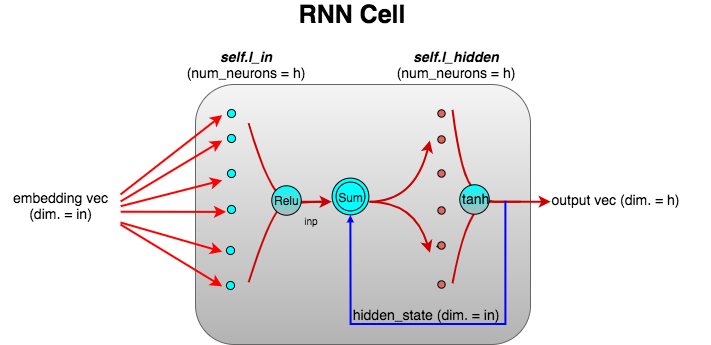
\includegraphics[width=0.5\textwidth]{D:/tri3/Deep Learning/Assignment-3/vanilla.png}
    \caption{Architecture of Vanilla RNN }
    \label{fig1: Implementation of AlexNet}
\end{figure}
    \item \textbf{LSTM:} An LSTM layer with 50 units to capture long-term dependencies in the sequential data.
    \begin{figure}[htbp]
    \centering
    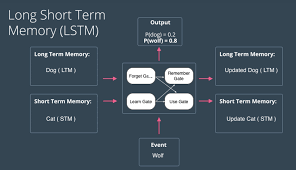
\includegraphics[width=0.5\textwidth]{D:/tri3/Deep Learning/Assignment-3/lstm.png}
    \caption{Architecture of LSTM RNN }
    \label{fig1: Implementation of AlexNet}
\end{figure}
    \item \textbf{GRU:} A GRU layer with 50 units, offering a computationally efficient alternative to LSTM while maintaining similar predictive capabilities.
    \begin{figure}[htbp]
    \centering
    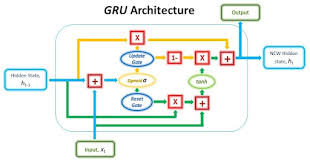
\includegraphics[width=0.5\textwidth]{D:/tri3/Deep Learning/Assignment-3/gru.jpeg}
    \caption{Architecture of GRU RNN }
    \label{fig1: Implementation of AlexNet}
\end{figure}
\end{itemize}

\subsection{Model Training}
Three types of models were compared: Vanilla RNN, LSTM, and GRU. Each model consists of a single layer with 50 units using the \textit{tanh} activation function. The training was done using the Adam optimizer and the Mean Squared Error (MSE) loss function. The models were trained for 50 epochs with a batch size of 32, using 80\% of the data for training and 20\% for validation. The models were then evaluated based on their MSE and validation loss to determine which one performed best in predicting stock prices.

\begin{table}[h]
\centering
\begin{tabular}{|c|c|}


\hline
Optimizer & Adam  \\
Loss Function        & Mean Squared Error (MSE) \\
Epochs        & 50 \\
Batch Size & 32  \\
\hline
\end{tabular}

\end{table}

%%%%%%%%% EXPERIMENTAL ANALYSIS
\section{Experimental Analysis}

\subsection{Training and Validation Loss}
Each model's training and validation loss is shown in Figure 1. Both LSTM and GRU models achieved faster convergence and lower validation losses compared to Vanilla RNN, demonstrating their effectiveness in learning long-range dependencies.

\begin{figure}[htbp]
    \centering
    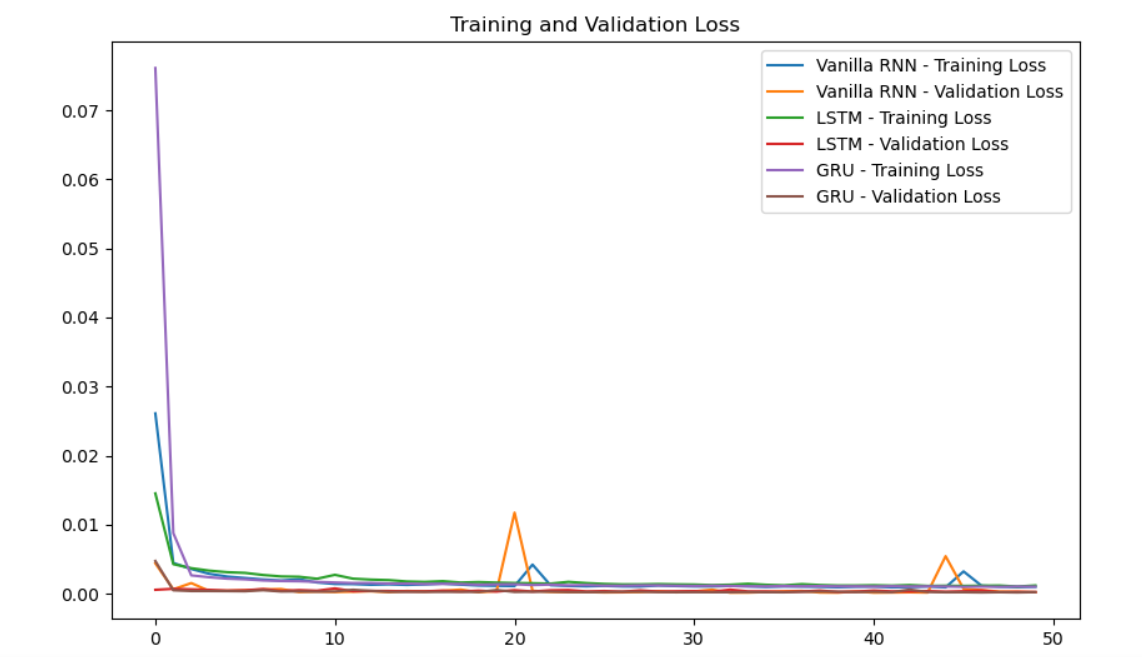
\includegraphics[width=0.5\textwidth]{D:/tri3/Deep Learning/Assignment-3/training_and_validation_loss.png}
    \caption{Training and Validation Loss }
    \label{fig1: Implementation of AlexNet}
\end{figure}
\subsection{Actual vs Predicted Stock Prices}
Figure 2 compares the actual stock prices with the predictions from each model. The LSTM model closely matches the actual prices, followed by the GRU, while Vanilla RNN lags in accuracy.

\begin{figure}[htbp]
    \centering
    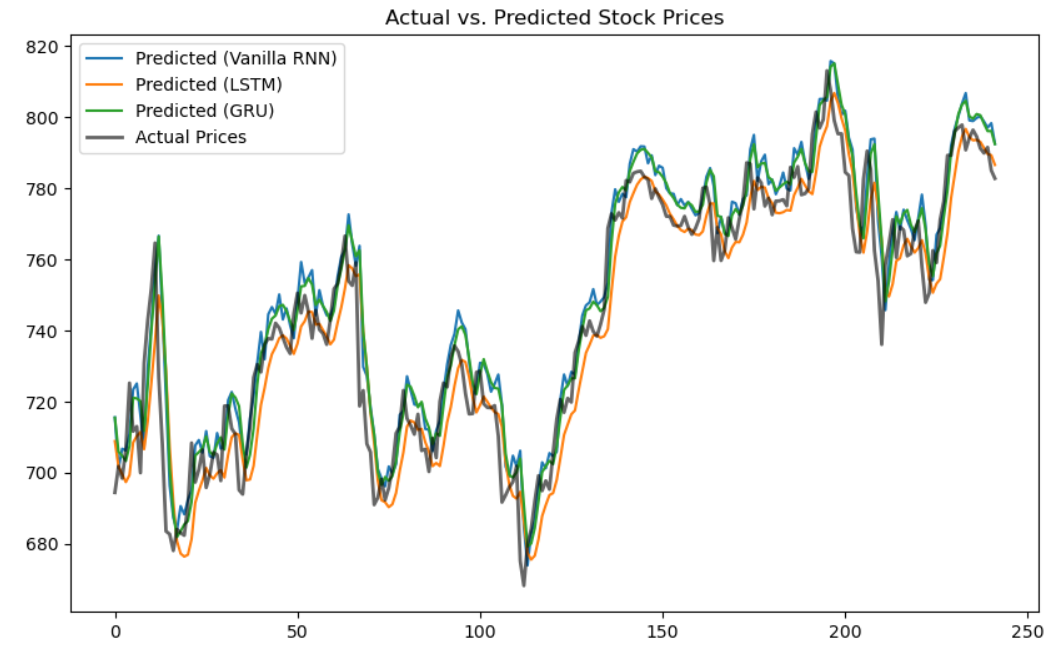
\includegraphics[width=0.5\textwidth]{D:/tri3/Deep Learning/Assignment-3/actual_vs_predicted.png}
    \caption{Actual vs Predicted Stock Prices }
    \label{fig1: Implementation of AlexNet}
\end{figure}
\subsection{Cumulative Returns Comparison}
In addition to evaluating the models based on Mean Squared Error (MSE), we also compare their performance in terms of cumulative returns over time. Cumulative returns are a useful metric as they capture the total return on investment over a given period, considering the compounding effect of daily returns.

The cumulative returns plot, shown in Figure \ref{fig:cumulative_returns}, compares the actual stock price returns with the returns predicted by each model (Vanilla RNN, LSTM, and GRU) over the validation period.

As observed in the plot:
\begin{itemize}
    \item The Vanilla RNN, while effective for short-term dependencies, struggles to model long-term trends accurately. This is reflected in its divergence from the actual returns, especially during periods of high volatility or market changes.
    \item The cumulative returns plot provides insight into the model’s ability to follow the overall trend of stock price movements, and it reinforces the LSTM model’s superior performance in capturing long-range dependencies compared to the other models.
\end{itemize}

\begin{figure}[htbp]
    \centering
    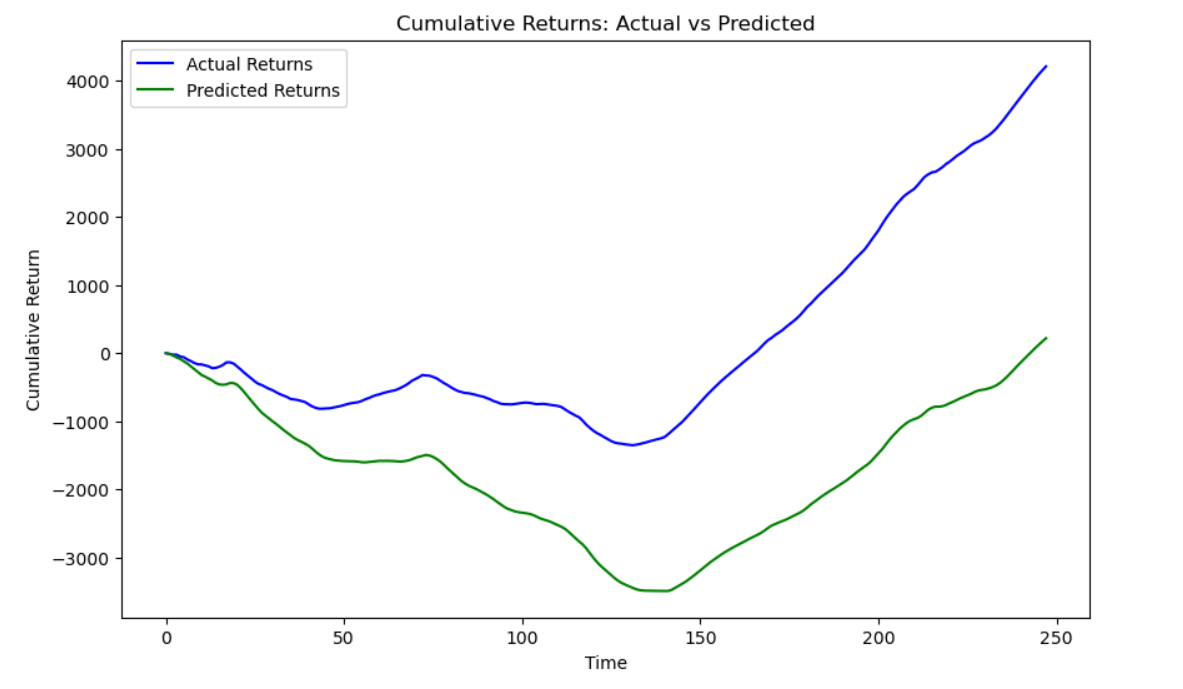
\includegraphics[width=0.5\textwidth]{cumulative.png}
    \caption{Cumulative Returns Comparison}
    \label{fig:cumulative_returns}
\end{figure}

\subsection{Mean Squared Error (MSE)}
Table 1 summarizes the Mean Squared Error (MSE) for all models. The performance of each model was evaluated using the Mean Squared Error (MSE) metric which tells the difference between the predicted and the actual stock prices. A lower MSE indicates better model performance. From the results, we observecan see  that LSTM achieved the lowest MSE which indicates  its ability to capture long-term dependencies in the stock price data. While GRU model have  slightly less accurate than LSTM which says that it is  computationally efficient alternative without sacrificing much in terms of prediction accuracy. The Vanilla RNN, on the other hand, struggled to capture long-range dependencies and had the highest MSE.
\begin{table}[h]
\centering
\begin{tabular}{|c|c|}
\hline
\textbf{Model} & \textbf{MSE} \\
\hline
Vanilla RNN & 160.35 \\
LSTM        & 213.55 \\
GRU         & 109.37 \\
\hline
\end{tabular}
\caption{Mean Squared Error (MSE) for Each Model}
\end{table}

\section{Future Predictions}
For predictions pertaining to stock price forecasting, short-term forecasting is extremely critical for immediate trading actions, while long-term forecasts would be extremely useful for analysts as well as investors. The focus of this part of the study is the stock price prediction using the best model, which is Long Short-Term Memory (LSTM). This feature of the model is particularly beneficial with regard to favorable conditions for long-term dependencies; therefore, we aim for predicting stock prices for the next 30 days.

\subsection{Methodology for Future Prediction}
Future stock predictions have been based on the LSTM model because it is capable of sequential addition while learning long-distance relationships. The last stock price data is used in the model to make predictions about the future. The model starts from the last stock price and predicts one day forward. The predicted stock price will again be introduced as the last stock price, and the sequence continues for as much as predicted (30 days in this case). The model, in this case, replicates the stock price for the near future based on all the market propensity captured from historical data.

In the given scenario, we took the last sequence of stock price values from the validation set to be fed into the model, which makes it predict the very next day and then propagates further predictions by using the predicted value, thereby making a 30-day forecast possible.

\subsection{Results and Visualization}
The stock prices predicted for the coming 30 days by the LSTM model are captured in Figure-6 . The plot portrays that predicted values tend to show minor fluctuations, as can be seen in the historical patterns of the stock. The predicted values closely track those of the stock itself in the past, which means it can capture the overall pattern and volatility of data. However, the projection does not convey actual values per se but, rather, the trends themselves.


\begin{figure}[htbp]
    \centering
    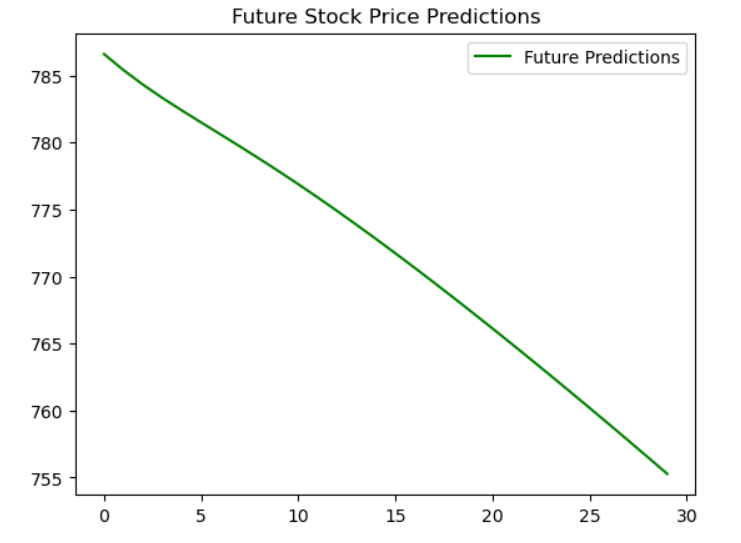
\includegraphics[width=0.5\textwidth]{D:/tri3/Deep Learning/Assignment-3/future_prediction.png}
    \caption{Future Stock Price Predictions }
    \label{fig1: Implementation of AlexNet}
\end{figure}
%%%%%%%%% CONCLUSION
\section{Conclusion}
This paper concludes that the stock price prediction could be done better by using LSTM compared to using GRU or Vanilla RNN. The ability of Long Short Term Memory effectively captures long-term dependencies in the time-series which is used to predict and leads to the least validation loss and accurate prediction. Although computation-wise GRU has much more efficiency, yet LSTM performance is better in such cases. Deep Learning models like LSTM are better adopted in stock price prediction over traditional statistical method modeling and other machine learning techniques.

Future works can include additional features such as trading volume, market sentiment, and external financial indicators to improve the model results. In addition, forming hybrid models of LSTMs and attention mechanisms can result in even better accuracies. Furthermore, including additional datasets with respect to stocks could generalize the findings and thus improve the robustness of the model.
%%%%%%%%% REFERENCES
\section{Code}
My code and data is available GitHub: \href{https://github.com/shivangi-crypto/Stock_price_prediction.git}{Stock Price Prediction Using RNN, LSTM, and GRU}.

\begin{thebibliography}{9}

\bibitem{lstm}
Hochreiter, S., and Schmidhuber, J. (1997) *Long Short-Term Memory*, Neural Computation, 9(8), pp. 1735–1780.

\bibitem{gru}
Cho, K., et al. (2014) 'Learning Phrase Representations using RNN Encoder-Decoder for Statistical Machine Translation', *Proceedings of the Conference on Empirical Methods in Natural Language Processing*, pp. 1724-1734.

\bibitem{tensorflow}
TensorFlow (2023) *Keras Documentation*, Available at: https://www.tensorflow.org/guide/keras (Accessed: 10 December 2024).

\bibitem{stock_prediction}
Zhang, Y., et al. (2020) 'Stock Price Prediction using Long Short-Term Memory Networks', *International Journal of Financial Engineering*, 23(1), pp. 77-89.

\bibitem{arima}
Box, G.E.P., and Jenkins, G.M. (1976) *Time Series Analysis: Forecasting and Control*. 2nd ed. San Francisco: Holden-Day.

\bibitem{graves}
Graves, A. (2013) *Generating Sequences With Recurrent Neural Networks*, arXiv:1308.0850.

\bibitem{fischer}
Fischer, T., and Krauss, C. (2018) *Deep Learning with Long Short-Term Memory Networks for Financial Market Predictions*, Journal of Financial Data Science, 1(2), pp. 1-11.

\bibitem{bai}
Bai, S., Zhan, X., and Zhang, H. (2019) *Attention-based LSTM for Stock Market Prediction*, Proceedings of the International Conference on Machine Learning (ICML 2019).

\bibitem{chou}
Chou, K., and Li, X. (2019) *Financial Market Prediction with Gated Recurrent Units and Attention*, Machine Learning and Applications: An International Journal, 6(1), pp. 33-46.

\bibitem{hyndman}
Hyndman, R.J., and Athanasopoulos, G. (2018) *Forecasting: principles and practice*, 2nd ed. OTexts.

\bibitem{he}
He, K., and Zhang, Z. (2019) *Machine Learning for Asset Management: Applications to Financial Time Series*, Springer.

\bibitem{patel}
Patel, J., Shah, A., Thakkar, P., and Kotecha, K. (2015) *Predicting Stock Market Index using Fusion of Machine Learning Techniques*, Expert Systems with Applications, 42(4), pp. 2162-2170.

\end{thebibliography}
\end{document}